\input{text/diss}

\begin{document}

\def\labauthors{Есюнин Д.В., Есюнин М.В.}
\def\labgroup{440}
\def\labnumber{1}
\def\labtheme{Измерение статистических характеристик полупроводникового диода}
\renewcommand{\vec}{\mathbf}
\renewcommand{\phi}{\varphi}
\renewcommand{\hat}{\widehat}

\input{text/titlepage}

\section{Введение}
Физика контактных явлений служит основой разработки важнейших структурных элементов подавляющего большинства приборов современной микроэлектроники. В данной работе будут кратко изучены элементарные основы теории контактных явлений как на границе двух различных материалов, так и внутри одного и того же полупроводникового кристалла между областями с разным типом проводимости. Физические свойства подобных контактов широко используются для выпрямления тока и лежат в основе работы базовых элементов целого ряда полупроводниковых сверхвысокочастотных устройств и быстродействующих интегральных схем, а также полупроводниковой оптоэлектроники.

\section{Границы раздела между полупроводниками}
\subsection{Изотипный (униполярный) гомопереход}
Область электронного полупроводника, имеющую высокую концентрацию доноров, обозначают $"n^+"$. Если в полупроводнике n-типа создается область $n^+$, то говорят об $n^+-n$ переходе. 

Поскольку концентрация электронов в $n^+$ области больше, чем в n-области, то диффузионный ток будет направлен справа налево (рис.1). Он будет переносить электроны, пока не возникнет внутреннее поле (образованное ионами доноров и избыточными электронами) такой величины, при которой создаваемый им встречный дрейфовый ток не уравновесит ток диффузионный, т.е. пока не будет достигнуто динамическое равновесие. Зонная диаграмма и графики зависимости концентрации доноров и электронов от координаты в равновесном состоянии показаны на рис.1. 
\begin{figure}[h!]
	\centering
	\includegraphics[width=0.35\linewidth]{fig/fig1.jpg}
	\caption{Энергетическая зонная диаграмма и график зависимостей концентрации доноров и электронов от координаты в $n^+-n$ переходе в состоянии равновесия}
	\label{fig:1}
\end{figure}

На практике чаще всего используют изотипные переходы с уровнями легирования обеих частей более $10^{16}-10^{17} \text{см}^{-3}$, поэтому высота барьера между правой и левой областями перехода имеет величину порядка нескольких kT, а электрическое сопротивление, обусловленное таким барьером, мало по сравнению с сопротивлениями остальных переходов.  
\subsection{Анизотипный (биполярный) гомопереход (p-n переход)}
Электронно-дырочным или p=n переходом называется приконтактная область между частями полупроводника с электронной (n)и дырочной (p) проводимостями. 

В зависимости от характера распределения примесей различают резкий (ступенчатый) и плавный p-n переходы. Рассмотрим резкий переход при условии $N_a \gg N_d$.

\subsubsection{Электронно-дырочный переход в равновесном состоянии}
В p-области концентрация дырок ($p_p$) - основных носителей заряда - значительно больше, чем в n-области. Поэтому они диффундируют в n-область, где будут неосновными носителями заряда ($p_n$). Благодаря интенсивной рекомбинации в некотором слое n-области, примыкающем к границе раздела, появится положительный объемный заряд, обусловленный ионами донорной примеси. Аналогично, диффузия и рекомбинация электронов будут сопровождаться образованием в p-области отрицательного объемного заряда ионов акцепторной примеси. Наличие объемного заряда вызывает появление встроенного электрического поля. Таким образом, на границе раздела между p- и n-областями появляется разность потенциалов, которую называют контактной $U_k$.

Электрическое поле, созданное в объединенной области ионами легирующей примеси, препятствует переходу через нее основных носителей заряда. Однако, это поле вызывает дрейфовый ток неосновных носителей, который направлен противоположно диффузионному току. В равновесном состоянии в отсутствие внешнего напряжения результирующий ток через переход равен нулю. Это означает, что силы электрического поля и силы, определяющее диффузию носителей заряда, уравновешивают друг друга. приконтактную область, где имеется электрическое поле, называют p-n переходом.

\subsubsection{Вольт-амперная характеристика p-n перехода}
Пусть к электронно-дырочному переходу подключен источник ЭДС таким образом, чтобы потенциальный барьер уменьшился. Такое подключение называется прямым и оно соответствует подсоединению источника плюсом к p-области и минусом к n-области. 

При прямом смещении из-за уменьшения потенциального барьера основные носители в областях p и n, имеющие наибольшую энергию, получат возможность преодолевать потенциальный барьер и проникать через него в области, где они оказываются неосновными и рекомбинируют. Эти избыточные неравновесные носители нарушат электронейтральность полупроводника вблизи перехода и вызовут в равном количестве приток основных носителей из глубины p- и n-областей. Скорость рекомбинации электронов и дырок конечна, поэтому неравновесные носители могут подвинуться вглубь полупроводника и глубина их проникновения значительно превысит толщину запорного слоя. При этом электронейтральность кристалла за пределами области объемного заряда не нарушается. 

Таким образом, при наложении внешнего напряжения в прямом направлении в результате инжекции  носителей через p-n переход будет протекать ток, величина которого будет нарастать с увеличением приложенного напряжения. при обратной полярности внешнего напряжения высота потенциального барьера увеличивается. Ток в этом случае определяется неосновными носителями заряда и незначителен по величине.

Вольт-амперная характеристика диода:
\begin{figure}[h!]
	\centering
	\includegraphics[width=0.5\linewidth]{fig/fig2.jpg}
	\caption{ВАХ p-n перехода: 1) идеальная; 2) реальная}
	\label{fig:2}
\end{figure}

Отличия от теоретической зависимости наблюдаются при увеличении прямого тока и при больших обратных напряжениях, когда имеет место резкое возрастание обратного тока и пробой перехода. 

У реального диода последовательно с сопротивлением p-n перехода имеется сопротивление базы (область с большей концентрацией примесей называют эмиттером, а с меньшей - базой). При больших прямых токах падение напряжения на этом сопротивлении соизмеримо с падением на переходе. С учетом сопротивления базы аналитическое выражение зависимости тока диода от приложенного к нему напряжения может быть представлено в виде:

\begin{gather}
	J=J_s[e^{(U/\varphi_T-JR_{\text{б}}/\varphi_T)}-1].
\end{gather}
где U - напряжение, приложенное к диоду, $R_{\text{б}}$ - сопротивление базы. 

Проведя логарифмирование и дифференцирование этого выражения, определим дифференциальное сопротивление в произвольной точке вольт-амперной характеристики:
\begin{gather}
	R_{\text{д}}=\dv{U}{J}=\frac{\varphi_T}{(J+J_s)}+R_{\text{б}}.
\end{gather}

Отсюда следует, что при малых токах дифференциальное сопротивление зависит главным образом от сопротивления p-n перехода. При больших токах дифференциальное сопротивление перехода мало и общее сопротивление определяется сопротивлением базы, т.е. зависимость от напряжения представляет собой линию, угол наклона которой пропорционален величине $R_{\text{д}}$. При дальнейшем увеличении прямого напряжения ток прибора выходит на насыщение. Причины этого явления зависят от конструкции прибора и определяются: насыщением зависимости скорости носителей заряда в сильных электрических полях, малой концентрацией носителей заряда при слабом легировании полупроводника, разогревом полупроводника протекающим током.

\subsubsection{Емкость электронно-дырочного перехода}
Всякий p-n переход по существу представляет собой систему двух проводников, разделенных слоем объемного заряда. Такая система подобна плоскому конденсатору. Опыт показывает, что полупроводниковые диоды обладают значительной емкостью. Емкость диода играет большую роль, ограничивая применение диодов на высоких частотах. изучение емкости перехода во многих случаях помогает исследовать структуру запирающего слоя и механизм выпрямления.

Ширина области объемного заряда:
\begin{gather}
	d=\sqrt{\frac{2\varepsilon \varepsilon_o(N_a+N_d)(U_k-U)}{eN_aN_d}}.
\end{gather} 

Видно, что ширина уменьшается с увеличением прямого (положительного) напряжения и увеличивается при обратном напряжении.

Изменение ширины области объемного заряда в связи с изменением напряжения приводит к изменению заряда в p- и n-областях. Поэтому p-n переход ведет себя подобно емкости. Эту емкость называют барьерной, т.к. она связана с образованием потенциального барьера между p- и n-областями. 
\begin{gather}
	C=S\frac{\varepsilon \varepsilon_o}{d}=S\sqrt{\frac{e\varepsilon \varepsilon_oN_aN_d}{2(N_a+N_d)(U_k-U)}},
\end{gather}
где S - площадь перехода.

В случае резко несимметричного p-n перехода, например, при $N_a \gg N_d$, переход расширяется в n-область и величина барьерной емкости не зависит от свойств p-области:
\begin{gather}
	C=S\sqrt{\frac{e\varepsilon \varepsilon_oN_d}{2(U_k-U)}}.
\end{gather}

Это выражение позволяет найти контактную разность потенциалов и концентрацию донорной примеси. График зависимости $\frac{1}{C^2}=f(U)$, изображенный на рис.3, отсекает на оси абсцисс отрезок, равный по величине $U_k$. Если известна зависимость $C=f(U)$, то на основании равенства (4) можно построить зависимость ширины объединенной области от приложенного напряжения.
\begin{figure}[h!]
	\centering
	\includegraphics[width=0.5\linewidth]{fig/fig3.jpg}
	\caption{Вольт-фарадная характеристика p-n перехода(здесь $U_{\text{обр}}$ - обратное напряжение).}
	\label{fig:3}
\end{figure}

\section{Эквивалентные схемы диодов}
\begin{figure}[h!]
	\centering
	\includegraphics[width=0.5\linewidth]{fig/fig4.jpg}
	\caption{Эквивалентная схема диодов на основе p-n перехода, барьера Шоттки и МПД структуры}
	\label{fig:4}
\end{figure}

Здесь С - управляемая напряжением емкость перехода; U - величина напряжения, приложенного непосредственно к переходу (т.е. без учета падения напряжения на сопротивлениях R1 и R2); R1 и R2 - последовательные сопротивления областей материала по обе стороны от перехода; $R_p$ - управляемое напряжением сопротивление перехода или барьера Шоттки (определяется из ВАХ диодов).

\section{Экспериментальная часть}
\subsection{Экспериментальная установка}
Схема:
\begin{figure}[h!]
	\centering
	\includegraphics[width=0.5\linewidth]{fig/fig5.jpg}
	\caption{Схема экспериментальной установки}
	\label{fig:5}
\end{figure}

$L=327\text{мкГн}$, $C_2$=33.8 пФ, S=1 мм$^2$.

Измерения статических характеристик полупроводникового диода (рис. 6) производится на установке, состоящей из блока режимов (1) и высокочастотного генератора (2).
\begin{figure}[h!]
	\centering
	\includegraphics[width=0.6\linewidth]{fig/fig6.jpg}
	\caption{}
	\label{fig:6}
\end{figure}

\subsection{ВАХ диода при комнатной температуре}
Сняли вольтамперную характеристику диода Д при комнатной температуре.

		
% Table generated by Excel2LaTeX from sheet 'Лист1'
\begin{table}[htbp]
	\centering
%	\caption{Add caption}
	\begin{tabular}{|c|c|c|c|c|c|c|c|c|c|c|c|c|c|c|}
		\toprule
		$I, \text{ мА}$ & 5     & 10    & 15    & 20    & 25    & 30    & 35    & 40    & 50    & 60    & 70    & 80    & 90    & 100 \\
		\midrule
		$U, 10^{-2} \text{ В}$ & 18    & 24    & 26    & 27    & 28    & 29    & 30    & 31    & 32    & 34    & 34    & 35    & 36    & 36 \\
		\midrule
		$I, \text{ мкА}$ & -16   & -17   & -18   & 19    & -20   & -21   & -22   &       &       &       &       &       &       &  \\
		\midrule
		$U, \text{ В}$  & -4    & -20   & -33   & -49   & -63   & -80   & -95   &       &       &       &       &       &       &  \\
		\bottomrule
	\end{tabular}%
%	\label{tab:addlabel}%
\end{table}%


\begin{figure}[H]
	\centering
	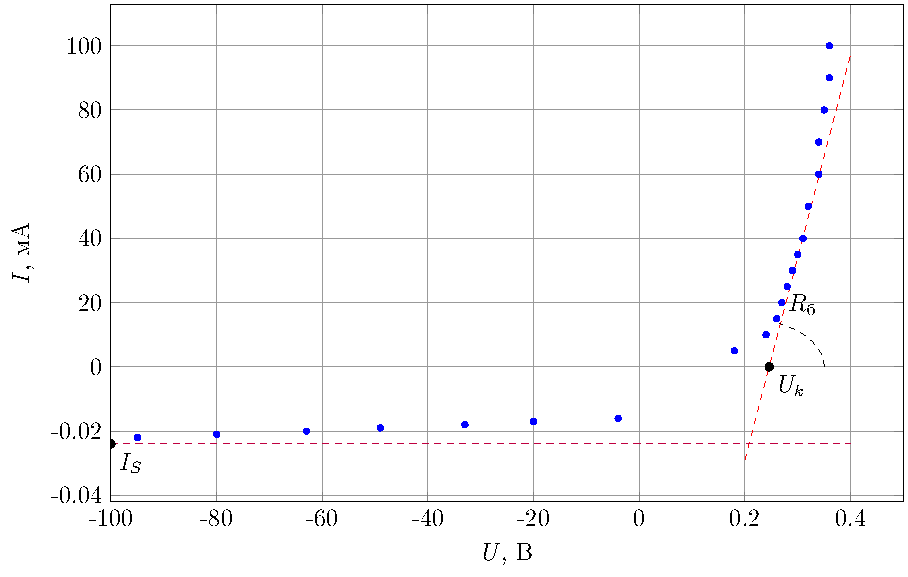
\includegraphics[width=\linewidth]{plots/plots1}
	\caption{вольтамперная характеристика диода при комнатной температуре}
	\label{fig:7}
\end{figure}
По данному графику могут быть вычислены контактная разность потенциалов $U_k$, а также величина тока насыщения $J_s$.
Измеренная ВАХ была аппроксимирована функцией (1), описывающей ВАХ идеального диода:
\begin{gather}
J=J_s[e^{(U/\varphi_T-JR_{\text{б}}/\varphi_T)}-1].
\end{gather}
Для аппроксимации данное уравнение не подходит, так как невозможно явным образом
выразить ток $J$ через напряжение $U$, поэтому выразим $U$ через $J$:
\begin{gather}
U=n\varphi_T\ln(\frac{J}{J_s}+1)+JR_{\text{б}}.
\end{gather}
Проведя аппроксимацию, получили следующие характеристики
$$n = 1.34, R_\text{б} = 0.84 \text{Ом}, J_s \approx -22 \text{ мкА}, U_k \approx 0.25 \text{ В}$$
\newpage
\subsection{Вольтфарадная характеристика диода}
Устанавливая различные смещения на диоде, искали резонансную частоту контура,
образованного емкостью диода Д, паразитной емкостью $C_2=33.8\text{ пФ}$ и катушкой индуктивности $L=327\text{ мкГн}$ для каждого значения смещения. Для определение емкости диода $C$ необходимо найти значение резонансной частоты контура
$$\nu=\frac{1}{2\pi\sqrt{LC_\text{общ}}}$$
где $C_\text{общ}=C+C_2$.
% Table generated by Excel2LaTeX from sheet 'Лист2'
\begin{table}[htbp]
	\centering
%	\caption{Add caption}
	\begin{tabular}{|c|c|c|c|c|c|c|c|c|}
		\toprule
		$U, \text{ В}$  & 0     & 6     & 12    & 18    & 24    & 30    & 36    & 42 \\
		\midrule
		$\nu, \text {МГц}$ & 0.578 & 1.367 & 1.392 & 1.406 & 1.411 & 1.422 & 1.424 & 1.433 \\
		\bottomrule
	\end{tabular}%
%	\label{tab:addlabel}%
\end{table}%

\begin{figure}[H]
	\centering
	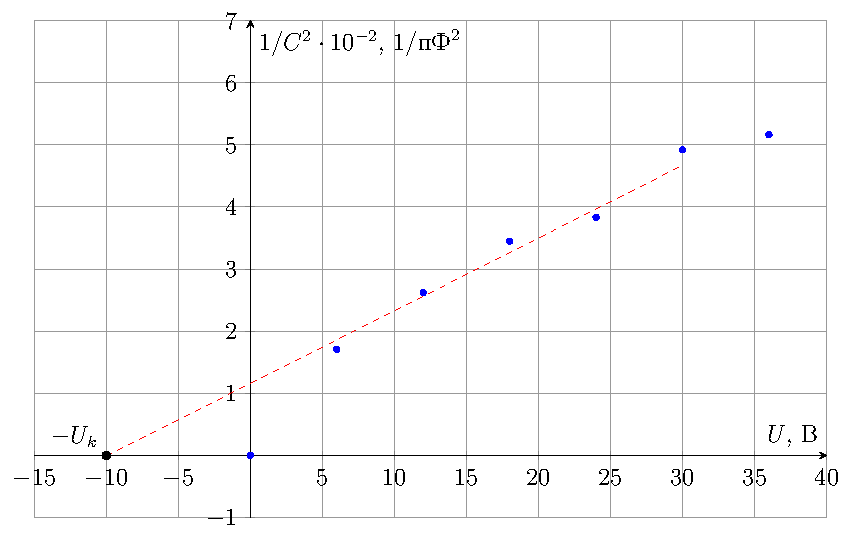
\includegraphics[width=\linewidth]{plots/plots2}
	\caption{вольтфарадная характеристика диода}
	\label{fig:8}
\end{figure}
Исходя из приведенного графика, можно найти значение контактной разности потенциалов $U_k=10\text{ В}$. Можно заметить, что полученное значение сильно отличается  от значения контактной разности потенциалов, полученной при исследовании ВАХ диода.
\subsection{ВАХ нагретого диода}
Сняли вольтамперную характеристику нагретого диода Д. Для этого включили режим измерения
обратной характеристики, установите напряжение $20…\ldots$ В, закрыли диод с нагревателем пенопластовой коробочкой, включите тумблер «Нагрев». Дождались, пока ток диода возрастет до 70...80 мкА, выключите нагреватель.
% Table generated by Excel2LaTeX from sheet 'Лист3'
\begin{table}[htbp]
	\centering
%	\caption{Add caption}
	\begin{tabular}{|c|c|c|c|c|c|c|c|c|c|c|c|}
		\toprule
		$I, \text{ мА}$ & 6     & 12    & 18    & 24    & 30    & 36    & 42    & 50    & 63    & 71    & 84 \\
		\midrule
		$U, 10^{-2} \text{ В}$ & 16    & 21    & 23    & 25    & 26    & 27    & 28    & 30    & 31    & 32    & 33 \\
		\midrule
		$I, \text{ мкА}$ & -62   & -70   & -75   & -79   & -84   & -90   &       &       &       &       &  \\
		\midrule
		$U, \text{ В}$  & -3    & -18   & -29   & -42   & -65   & -92   &       &       &       &       &  \\
		\bottomrule
	\end{tabular}%
%	\label{tab:addlabel}%
\end{table}%
\begin{figure}[H]
	\centering
	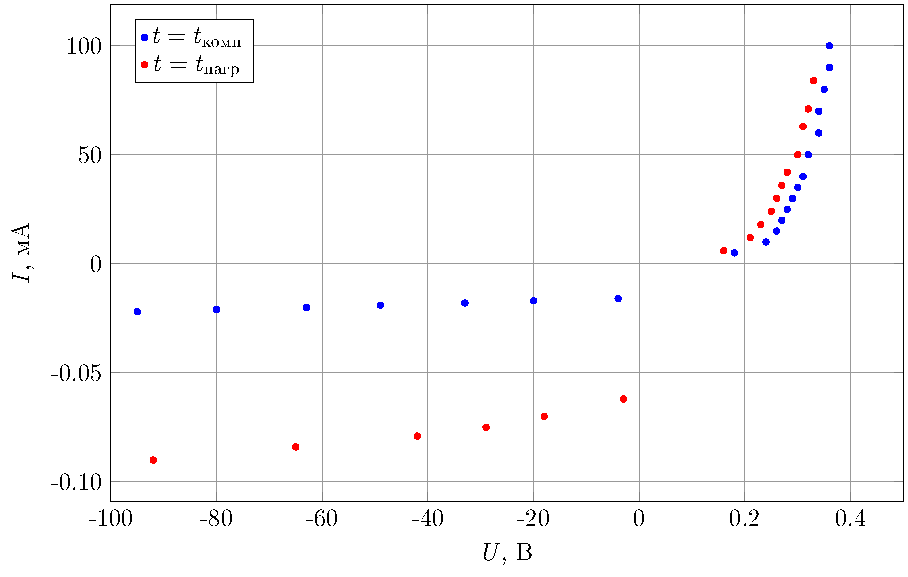
\includegraphics[width=\linewidth]{plots/plot4}
%	\caption{вольтамперная характеристика диода }
	\label{fig:10}
\end{figure}
\begin{figure}[H]
	\centering
	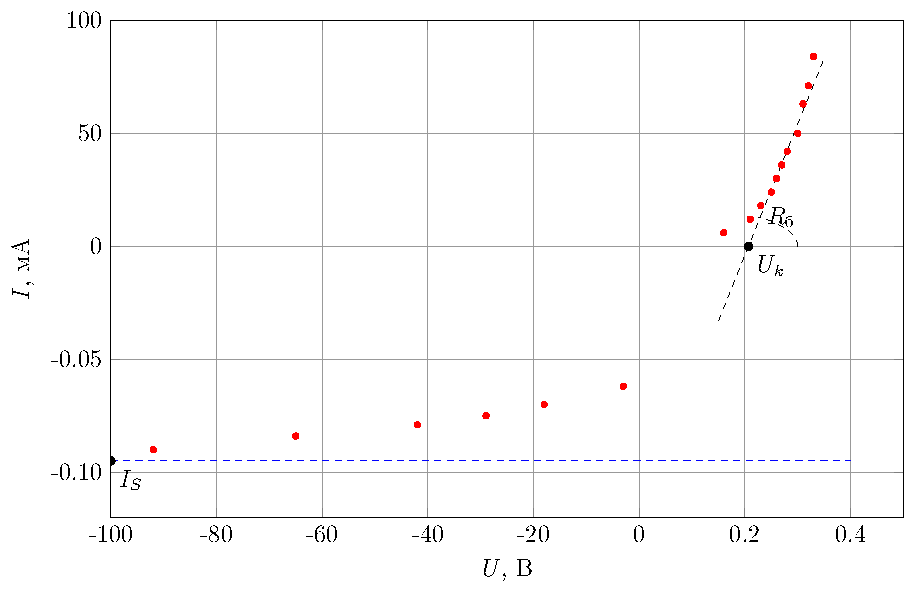
\includegraphics[width=\linewidth]{plots/plots3}
	\caption{вольтамперная характеристика диода при комнатной температуре}
	\label{fig:9}
\end{figure}
По данному графику могут быть вычислены контактная разность потенциалов $U_k$, а также величина тока насыщения $J_s$.

Проведя аппроксимацию, получили следующие характеристики
$$n = 2.34, R_\text{б} = 0.065 \text{Ом}, J_s \approx -95 \text{ мкА}, U_k \approx 0.20 \text{ В}$$
На графике ВАХ нагретого диода (рис. 9), также приведена ВАХ диода при комнатной температуре. Видно, что при повышении температуры ток насыщения увеличивается. Полученные результаты совпадают с теоретическими ожиданиями, так как обратный ток обусловлен тепловой генерацией неосновных носителей заряда в нейтральных $p$− и
$n$− областях, прилегающих к переходу. Носители проникают к границам перехода и переносятся в соседнюю область полем. При повышении температуры, скорость генерации
неосновных носителей возрастает, из-за чего увеличивается шанс прохождения последних
через границу перехода, увеличивая тем самым обратный ток.
\section{Вывод}
Были изучены принципы работы полупроводниковых устройств, а также уравнения описывающие явления, наблюдаемые в данной работе, сняты вольтамперные характеристики диода при разных значениях температур. Анализ показал, что при увеличении температуры диода величина тока насыщения увеличивается. При изучение вольтфарадной характеристики диода удалось экспериментально получить зависимость емкости диода от подаваемого напряжения смещения. 
\end{document}
